
\documentclass[a4paper, 11pt, oneside]{memoir}

%%%%% Packages %%%%%
\usepackage{lmodern}
\usepackage{palatino}
\usepackage[T1]{fontenc}
\usepackage[utf8]{inputenc}
\usepackage[french]{babel}


%%%%%%%%%%%%%%%%%%%% PACKAGE SECONDAIRE

% \usepackage{amstext,amsmath,amssymb,amsfonts} % package math
% \usepackage{multirow,colortbl}	% to use multirow and ?
% \usepackage{xspace,varioref}
\usepackage[linktoc=all, hidelinks]{hyperref}			% permet d'utiliser les liens hyper textes
\usepackage{float}				% permet d ajouter d autre fonction au floatant
% \usepackage{wrapfig}			% permet d avoir des image avec texte coulant a cote
% \usepackage{fancyhdr}			% permet d inserer des choses en haut et en bas de chaque page
\usepackage{microtype}			% permet d ameliorer l apparence du texte
%\usepackage[explicit]{titlesec}	% permet de modifier les titres
\usepackage{graphicx}			% permet d utiliser les graphiques
\graphicspath{{./images/}}		% to say where are image
% \usepackage{eso-pic} 			% to put figure in the background
\usepackage[svgnames]{xcolor}	% permet d avoir plus de 300 couleur predefini
% \usepackage{array}				% permet d ajouter des option dans les tableaux
% \usepackage{listings}			% permet d ajouter des ligne de code
% \usepackage{tikz}				% to draw figure
% \usepackage{appendix}			% permet de faire les index
% \usepackage{makeidx}			% permet de creer les index
% \usepackage{fancyvrb}			% to use Verbatim
% \usepackage{framed}				% permet de faire des environnement cadre
% \usepackage{fancybox}			% permet de realiser les cadres
%\usepackage{titletoc}			% permet de modifier les titres
\usepackage{caption}
\usepackage[a4paper, top=2cm, bottom=2cm]{geometry}
\usepackage[final]{pdfpages} 
\usepackage{eurosym}

\usepackage{graphicx}
\RequirePackage{pageGardeEnsta}	% permet d avoir la page de garde ensta

% \setcounter{secnumdepth}{2}		% permet d'augmenter la numerotation
% \setcounter{tocdepth}{2}		% permet d'augmenter la numerotation

%%%%%%%%%%%%%%%%%% DEFINITION DES BOITES
\newcounter{rem}[chapter]

\newcommand{\remarque}[1]{\stepcounter{rem}\noindent\fcolorbox{OliveDrab}{white}{\parbox{\textwidth}{\textcolor{OliveDrab}{
        \textbf{Remarque~\thechapter.\therem~:}}\\#1}}}

\newcounter{th}[chapter]

\newcommand{\theoreme}[2]{\noindent\fcolorbox{FireBrick}{white}{\stepcounter{th}
    \parbox{\textwidth}{\textbf{\textcolor{FireBrick}{Théorème~\thechapter.\theth~:}}{\hfill \textit{#1}}\\#2}}}

\newcommand{\attention}[1]{\noindent\fcolorbox{white}{white}{\parbox{\textwidth}{\textcolor{FireBrick}{
        \textbf{Attention !}}\\\textit{#1}\\}}}
%%%%%%%%%%%%%%%%%%%%%%%%%%%%%%%%%%%%%%%%%%%%%%%%%%%%%%%%%%%%%%%%%%%%%%%%% 


%% INDEX %%%%%%%%%%%%%%%%%%%%%%%%%%%%%%%%%%%%%%%%%%%%%%%%%%%%
\makeindex

%%%%% Useful macros %%%%%
\newcommand{\latinloc}[1]{\ifx\undefined\lncs\relax\emph{#1}\else\textrm{#1}\fi\xspace}
\newcommand{\etc}{\latinloc{etc}}
\newcommand{\eg}{\latinloc{e.g.}}
\newcommand{\ie}{\latinloc{i.e.}}
\newcommand{\cad}{c'est-à-dire }
\newcommand{\st}{\ensuremath{\text{\xspace s.t.\xspace}}}

%%%% Definition des couleur %%%%

\newcommand\couleurb[1]{\textcolor{SteelBlue}{#1}}
\newcommand\couleurr[1]{\textcolor{DarkRed}{#1}}


%% number page style style %%%%%%%%%%%%%%%%%%%%%%%%%%%%%%%%%%%%%%%%%%%%%%%%%%%%%%

\pagestyle{plain}
% \pagestyle{empty}
% \pagestyle{headings}
% \pagestyle{myheadings}



%% chapters style %%%%%%%%%%%%%%%%%%%%%%%%%%%%%%%%%%%%%%%%%%%%%%%%%%%%%%
%% You may try several styles (see more in the memoir manual).

% \chapterstyle{veelo}
% \chapterstyle{chappell}
% \chapterstyle{ell}
% \chapterstyle{ger}
% \chapterstyle{pedersen}
% \chapterstyle{verville}
\chapterstyle{madsen}
% \chapterstyle{thatcher}


%%%%% Report Title %%%%%
\title{Analyse fonctionnelle}
\author{Équipe Smart}
% \author{\textsc{Rigaud Michaël} \textsc{D'Acremont Antoine} \textsc{Cotten Guillaume} \textsc{Legay Kevin} \textsc{Aya Kenaan} \textsc{Mohamed Shehade}}
\date{\today}
\doctype{Rapport}
\promo{promo 2017}
\etablissement{\textsc{Ensta} Bretagne\\2, rue François Verny\\
  29806 \textsc{Brest} cedex\\\textsc{France}\\Tel +33 (0)2 98 34 88 00\\ \url{www.ensta-bretagne.fr}}
\logoEcole{
\includegraphics[height=4.2cm]{logo_ENSTA_Bretagne_Vertical_CMJN}}



%%%%%%%%%%%%%%%%%% DEBUT DU DOCUMENT
\begin{document}

\maketitle
\thispagestyle{empty}
\newpage

\tableofcontents

\newpage
%%%%%%%%%%%%%%%%% INTRODUCTION

\chapter*{Introduction}
\addcontentsline{toc}{chapter}{Introduction}

Ce document constitue le rapport de l'analyse fonctionnelle du projet Smart.
L'équipe Smart est constituée de Rigaud Michaël, D'Acremont Antoine, Cotten Guillaume, Legay Kevin, Aya Kenaan, et Mohamed Shehade.

Le projet Smart a pour but de mettre en place un système de détection et de neutralisation de drones.

Compte tenu du temps imparti, nous avons choisi de nous concentrer sur la détection d'un drone. Pour réaliser cette détection, nous utiliserons un ensemble de goniomètre permettant de réaliser la localisation d'un drone. Ce projet étant nouveau, l'ensemble des recherches et la réalisation du système devront être mené dans le temps imparti.

\newpage

%%%%%%%%%%%%%%%%%%%%%%%% 

\part{Analyse fonctionnelle}

%\chapter{État de l'art des technologies}

\chapter{Présentation du contexte}

L'actualité récente a montré que l'intrusion de drones dans des sites sécurisés représentaient un risque de sécurité majeur. Des gouvernements et entreprises privées se sont lancés dans la mise au point de systèmes de détection et de neutralisation de ces drones. Une recherche bibliographique nous a permis de mettre en évidence plusieurs méthodes de détection, pouvant être classées selon trois types principaux : acoustiques, optiques et électromagnétiques.  
Les paragraphes qui suivent détailleront les différents avantages et inconvénients que ces systèmes possèdent.

\section{Acoustique}

Plusieurs entreprises proposent des outils de détection acoustique des drones. Ces derniers se présentent sous forme de boîtiers reliés à des micros, positionnés en hauteur: c'est par les sons qu'ils génèrent, principalement ceux de leurs hélices, que les drones sont repérés et cela dans un rayon d'une centaine de mètres. Certains systèmes utilisent une analyse fréquentielle poussée du signal afin de détecter les moteurs en fonction de leurs fréquences de fonctionnement. Une alerte est alors envoyée à l'utilisateur du dispositif, sur un ordinateur ou par un SMS. L'avantage principal du système est qu'il peut détecter les drones n'émettant aucun rayonnement électromagnétique comme les systèmes auto-pilotés. Au-delà de cet aspect, il présente un avantage et des plus importants, son coût. En effet, un tel système est très économique à produire. Actuellement diverses solutions actives comme passives sont déjà présentes sur le marché et la démocratisation de ce type de système tends à faire baisser leur prix.

Toutefois ces appareils présentent certains défauts qui peuvent affecter leur fiabilité. Leur efficacité est en effet dépendante du bruit de fond qui doit être inférieur à un certain seuil pour que le système puisse détecter un drone. D'autres phénomènes acoustiques comme la réverbération du son et la présence d'échos peuvent aussi perturber son fonctionnement. Cela rend l'utilisation de telles solution difficile en milieu urbain. Enfin, il est nécessaire de disposer préalablement d'une base de données des signatures acoustiques des différents drones qui peuvent émettre sur un domaine de fréquences acoustiques larges. Il est assez simple pour un drone de parer ce système de détection. Par la simple émission d'une onde sonore couvrant sa propre signature acoustique, un drone passerait totalement inaperçu.

 Ces solutions sont orientées vers une utilisation domestique et non professionnelle pour les raisons évoquées précédemment. Leur prix se situe aux alentours de 100 dollars pour un modèle simple.

\section{Optique}

Une caméra normale a besoin de lumière pour produire une image, une caméra thermique (ou infrarouge) peut capter de très faibles différences de température et les convertir en une excellente image thermique sur laquelle les plus petits détails sont visibles. Contrairement à d'autres technologies, comme l'amplification de lumière qui nécessite une petite quantité de lumière pour produire une image, l'imagerie thermique permet de voir dans l'obscurité totale. Elle ne nécessite aucune source de lumière.

Depuis qu'il est possible de produire une image lisible dans l'obscurité totale, la technologie de l'imagerie thermique permet de voir et de cibler les forces ennemies dans la nuit la plus noire. Les caméras thermiques voient à travers la brume, la pluie et la neige. Elles voient aussi à travers la fumée, ce qui était particulièrement intéressant pour l'armée.\cite{optique}

En mode passif, \emph{des caméras thermiques d'observation savent repérer un drone de 50 cm d'envergure à une distance d'environ 1 km, de jour comme de nuit} . Lorsqu'un drone entre dans son champ de vision, des algorithmes identifient son image. La forme, la couleur et la géométrie de l'objet permettent de distinguer le drone d'éventuels oiseaux et lancer une alerte, à condition qu'il n'y ait pas d'obstacle entre la caméra et lui.

En mode actif, on peut éclairer une scène à $360^{\circ}$ avec un laser. \emph{Les photons, les particules de lumière, se réfléchissent sur l'appareil, le signal est récupéré et analysé.} D'une portée similaire à celle de la caméra, le laser a l'avantage de \emph{décamoufler} (observation à travers brouillard, pluie ou filet de camouflage), de livrer la distance précise de l'objet, et de le reconstituer en imagerie 3D.Une fois le drone suffisamment proche, une caméra \textit{classique} avec un opérateur humain peuvent prendre le relai pour vérifier visuellement la nature de l'intrus et éventuellement passer à la phase de neutralisation.

L'utilisation d'un caméra optique simple pourrait aussi convenir à condition d'utiliser un traitement d'image adapté. La complexité de ce traitement associé au nombres de formes de drones pouvant être acheté dans le commerce rends cette technique difficilement exploitable.


\section{Radar}
Le radar (de l'anglais RAdio Detection And Ranging) est un système qui utilise les ondes électromagnétiques pour détecter la présence d'objets. Le radar émet des ondes, elles rebondissent sur les objets rencontrés et il est possible de mesurer leur distance, la direction, l'altitude ainsi que la vitesse en analysant le signal renvoyé. Les modèles Doppler peuvent ainsi détecter les objets en mouvement : avion, hélicoptère et certains modèles de drones, même « légers ». C'est le cas du radar Squire de Thales Air Systems. 

~\\

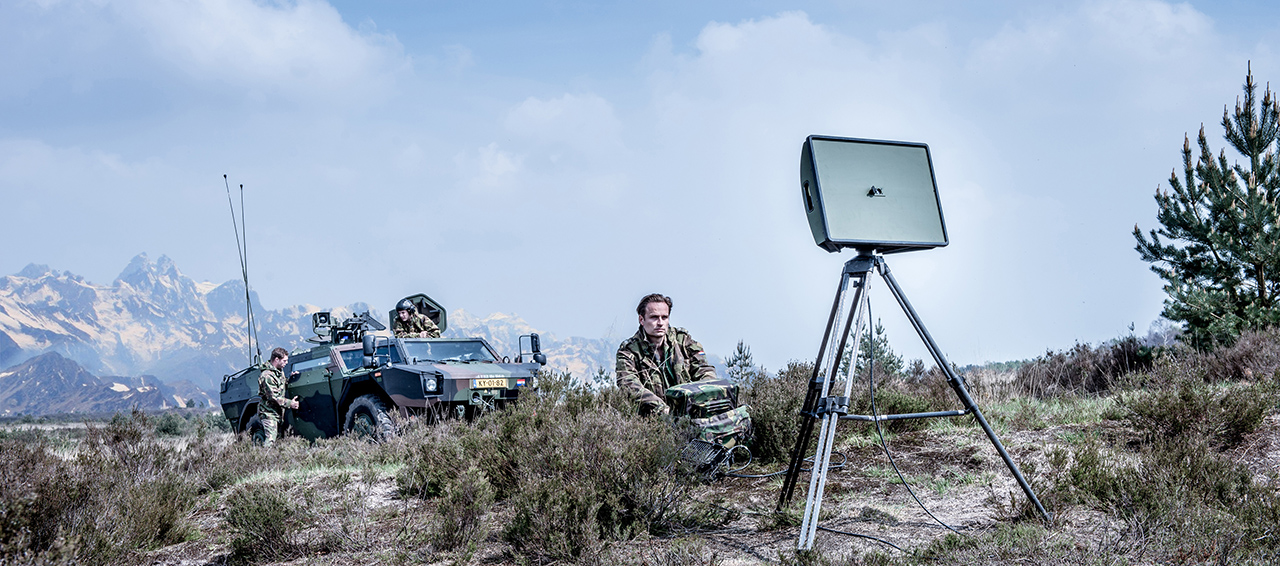
\includegraphics[width=\textwidth]{radar}
\captionof{figure}{Le radar portable Squire de Thales Air Systems}

Il existe néanmoins certains drones construits en carbone pouvant être perméables à certaines ondes radars et ainsi indétectable par cette technologie. Cependant le "radar passif", radar exploitant les variations d'ondes électromagnétiques en milieu urbain, telles que les ondes de la TNT, pourrait être exploité en milieu urbain.



\section{Radiogoniométrie}

Parmi les moyens existants pour détecter un drone on peut citer la radiogoniométrie. Le principe de la radiogoniométrie est de mesurer la direction d'arrivée d'une onde électromagnétique polarisée incidente sur un réseau de capteur, par rapport à une direction de référence. Les radio-goniomètres sont donc des détecteurs passifs. 

La radiogoniométrie possède de nombreuses applications. Cependant, en interception, la radiogoniométrie permet de localiser un émetteur inconnu soit en employant plusieurs récepteurs en des positions différentes, soit par calcul en fonction de la cinématique propre du récepteur. 

On distingue deux types de goniomètres: les goniomètres à une dimension qui n'estiment que le gisement ou l'azimut, et les goniomètres à deux dimensions qui estiment le gisement ou azimut ainsi que l'élévation. 


Dans le cas d'une détection de drones, le radio-goniomètre réalise une écoute de l'environnement avec un balayage de fréquences. Lorsque le drone émettra avec la personne qui le guide on pourra ainsi le localiser précisément.

L'avantage principal de la radiogoniométries est qu'il s'agit d'une méthode de détection passive. Elle est donc difficilement décelable et cela fait d'elle une technique fréquemment utilisée en guerre électronique. 

Seulement, la radiogoniométrie a des failles. En effet, il existe sur le marché des drones auto-pilotés qui n'émettent pas car ils chargent avant le début de leur vol leurs trajectoires. Ainsi il n'y a pas de communication avec un quelconque utilisateur, et donc il n'y a aucun signal émis. Il est donc impossible de les localiser à l'aide de cette technique.





\section{Synthèse}

Une solution technique idéal couplerait l'ensemble des méthodes décrites ci-dessus pour pouvoir parer à toute éventualité. Une analyse des solutions présentes sur le marché ou en développement montre que les configurations les plus performantes associent au moins deux des modes de détection cités. On peut notamment citer le cas du système drone-detector \cite{dronedetector}.

Néanmoins nous avons choisi pour ce projet de nous concentrer, dans un premier temps, sur une détection uniquement à base de radiogoniométrie.

Les raisons de ce choix sont les suivantes : Dans un premier temps, pour pouvoir réaliser un prototype fonctionnel il est plus aisé de se baser sur la radiogoniométrie compte tenu du matériel à notre disposition. Dans un second temps, notre équipe à choisi de se concentrer sur la détection de drones de loisir disponibles dans le commerce. Selon la réglementation ces drones doivent maintenir un lien radio avec un pilote qui doit être en mesure de reprendre le contrôle du drone à tout instant. Il y a donc une liaison permanente qui peut être exploitée par le système.




% Ici il va falloir préciser plusieurs choses sur pourquoi ce choix. Notamment en précisant qu'on suppose que les drones respectent la réglementation, etc... 



%%% Local Variables: 
%%% mode: latex
%%% TeX-master: "rapport_analyse"
%%% End: 

\chapter{Analyse fonctionnelle}

\section{Interview}

Après notre interview avec notre encadrant Ali Mansour, nous avons réalisé un tableau des spécifications suivantes:

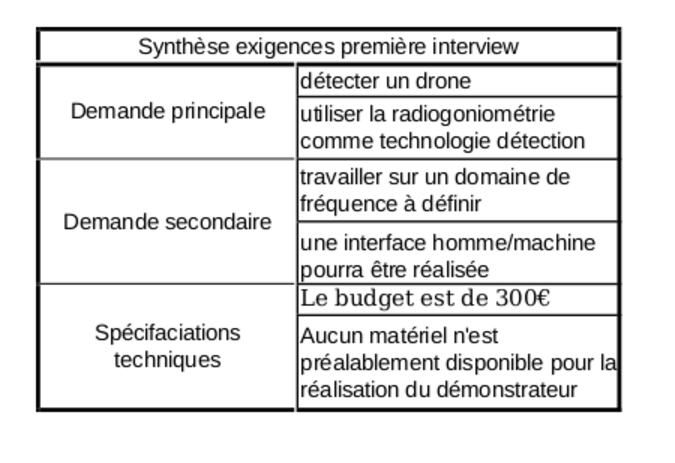
\includegraphics[width=0.8\textwidth]{interview}


\section{Tableau des spécifications}
En prenant en compte les recommandations de notre encadrant, et les recherches que nous avons réalisées, nous avons établi les contraintes et les spécifications suivantes:

%\includegraphics[width=\textwidth]{tableauSpe}
\includepdf{./images/tableauSpe.pdf}

%Compte tenu des recherches que nous avons réalisées, nous avons établi l'étude fonctionnelle suivante.

%De la synthèse de ce tableau découle le diagramme Pieuvre et les SADT suivant.

\section{Diagramme pieuvre}
~\\
~\\
~\\
~\\
~\\
~\\
\hspace{-2cm}
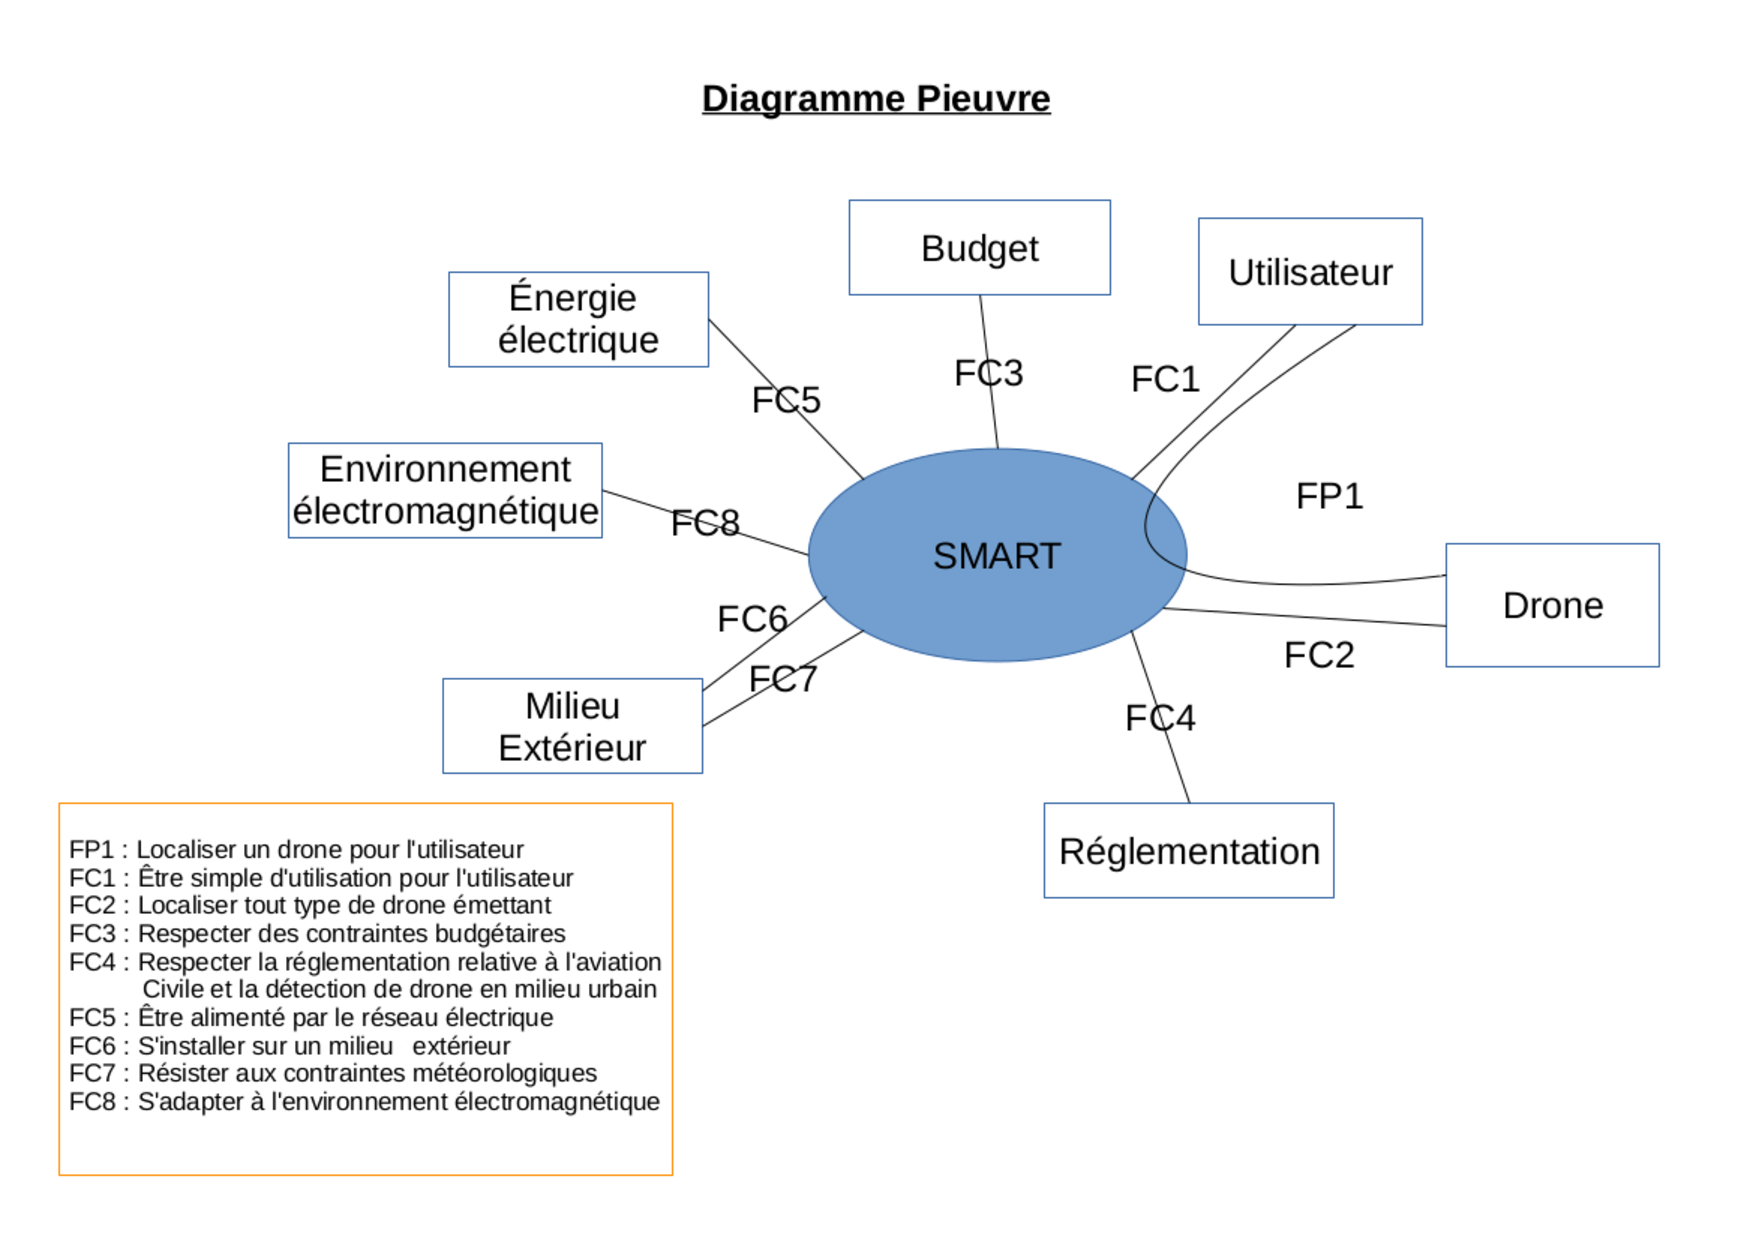
\includegraphics[width=1.18\textwidth]{Diagramme_pieuvre.pdf}
\captionof{figure}{Diagramme pieuvre}



\section{SADT}

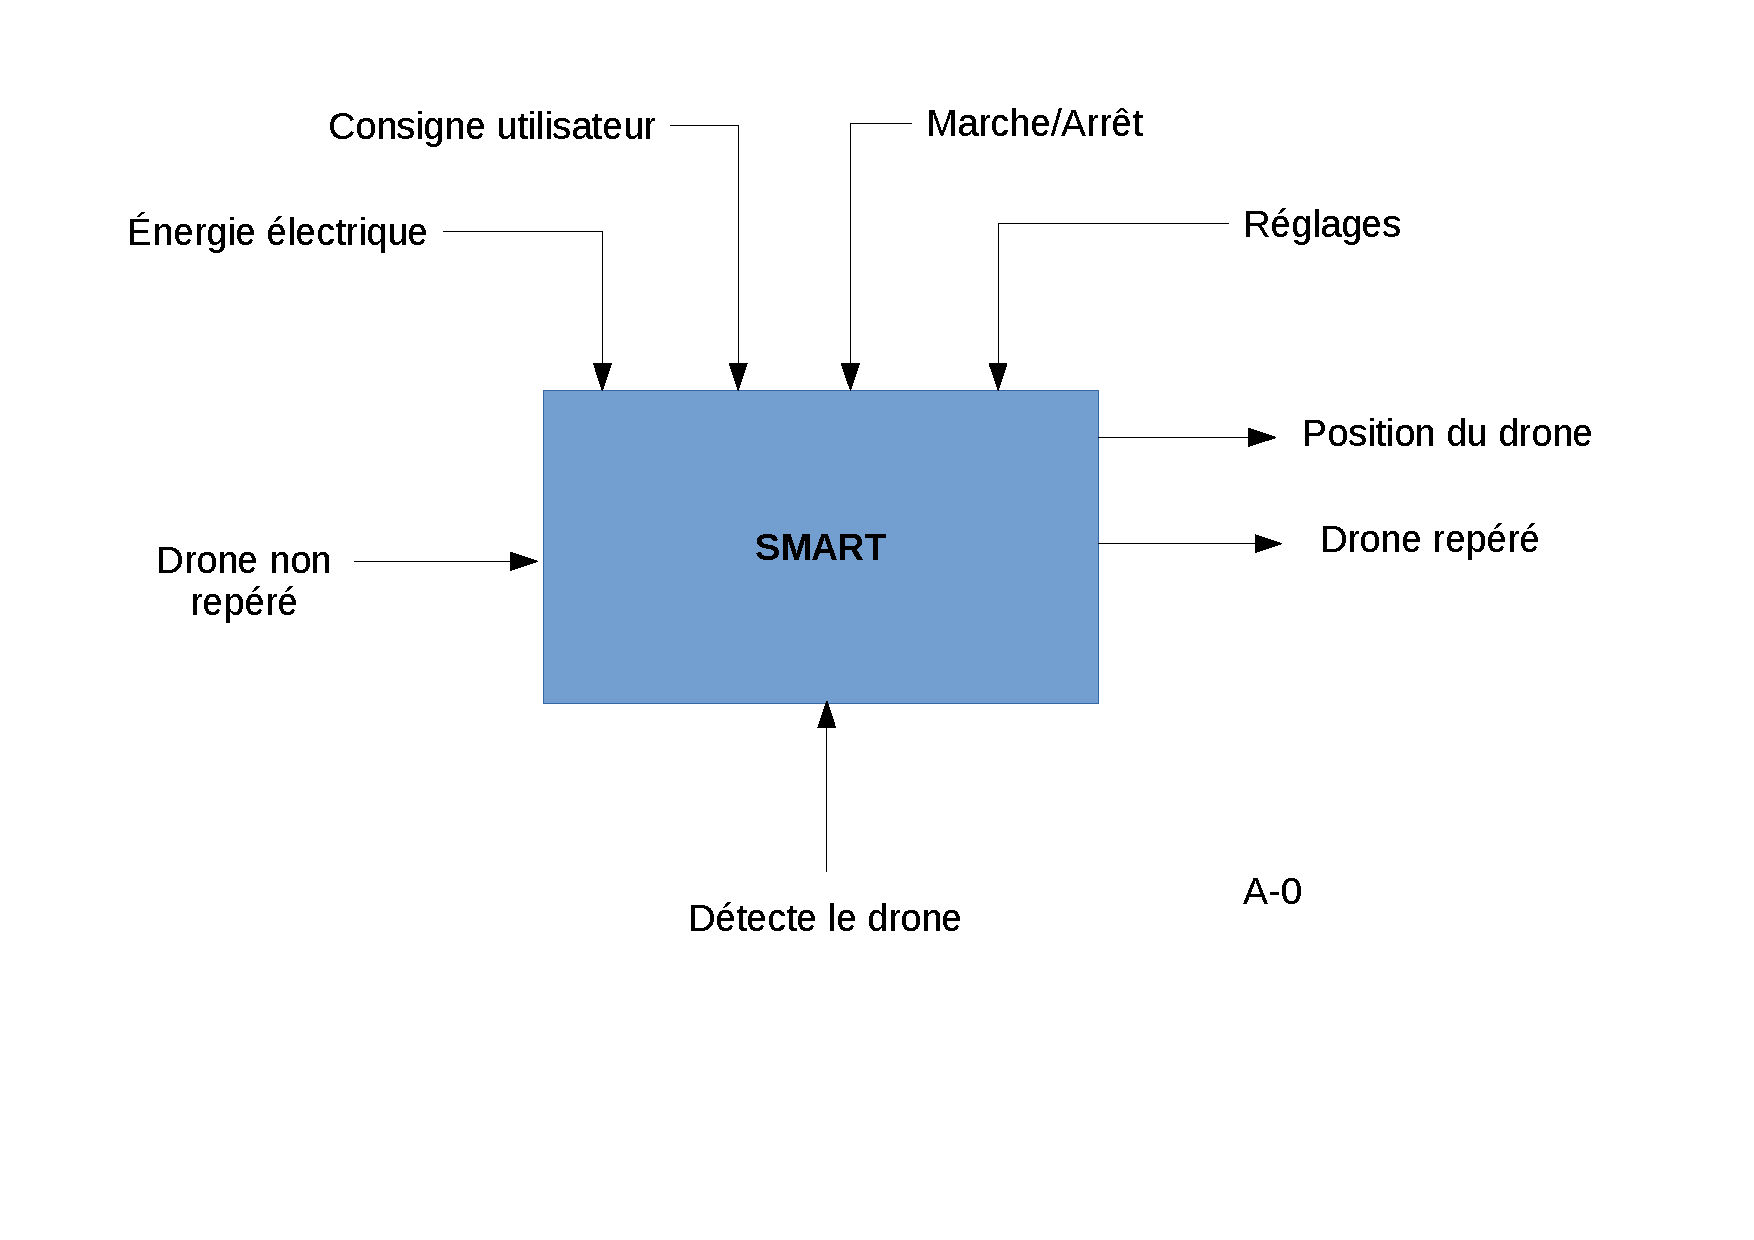
\includegraphics[width=\textwidth]{SADT_A-0.pdf}
\captionof{figure}{SADT A-0}
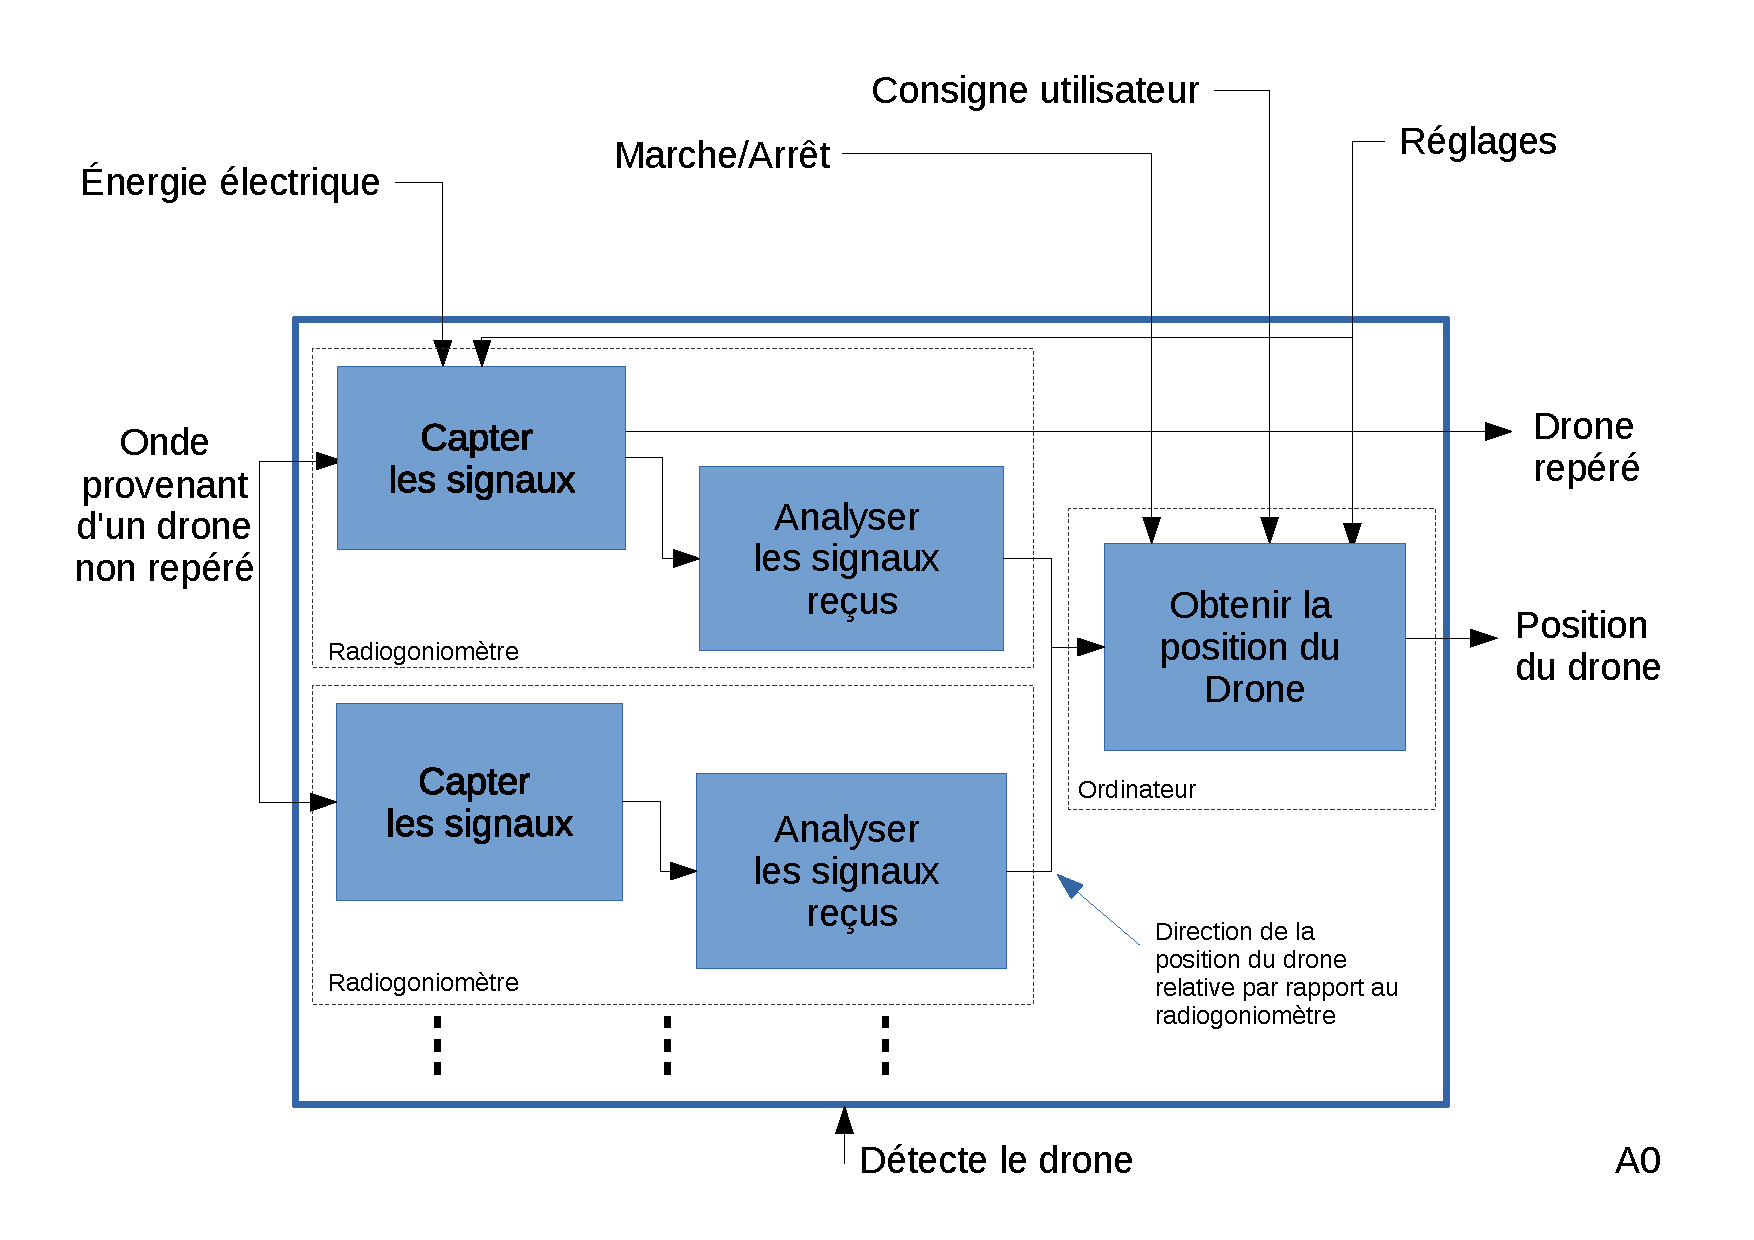
\includegraphics[width=\textwidth]{SADT_A0.pdf}
\captionof{figure}{SADT A0}

\newpage
\parindent=15pt

Comme on peut le voir sur le SADT A0, nous avons découpé notre objectif en trois parties.

Dans un premier temps il faut capter les signaux. Pour cela il faut réaliser un balayage sur le radiogoniomètre pour détecter les bons signaux.

Ensuite, il faut analyser les signaux reçus pour s'assurer que nous sommes bien en présence d'un drone.

Enfin, il faut récupérer les données des radiogoniomètres pour déterminer la position du drone.


\section{Fonctionnement de notre système}

Nous avons donc imaginé positionner plusieurs radiogoniomètres, chaque appareil indiquerait la direction du drone par rapport à sa position. Chacun d'eux serait connecté à un ordinateur central qui analyserai chacune des positions données par les radiogoniomètres et en déduirait la position du drone dans l'espace.

~\\

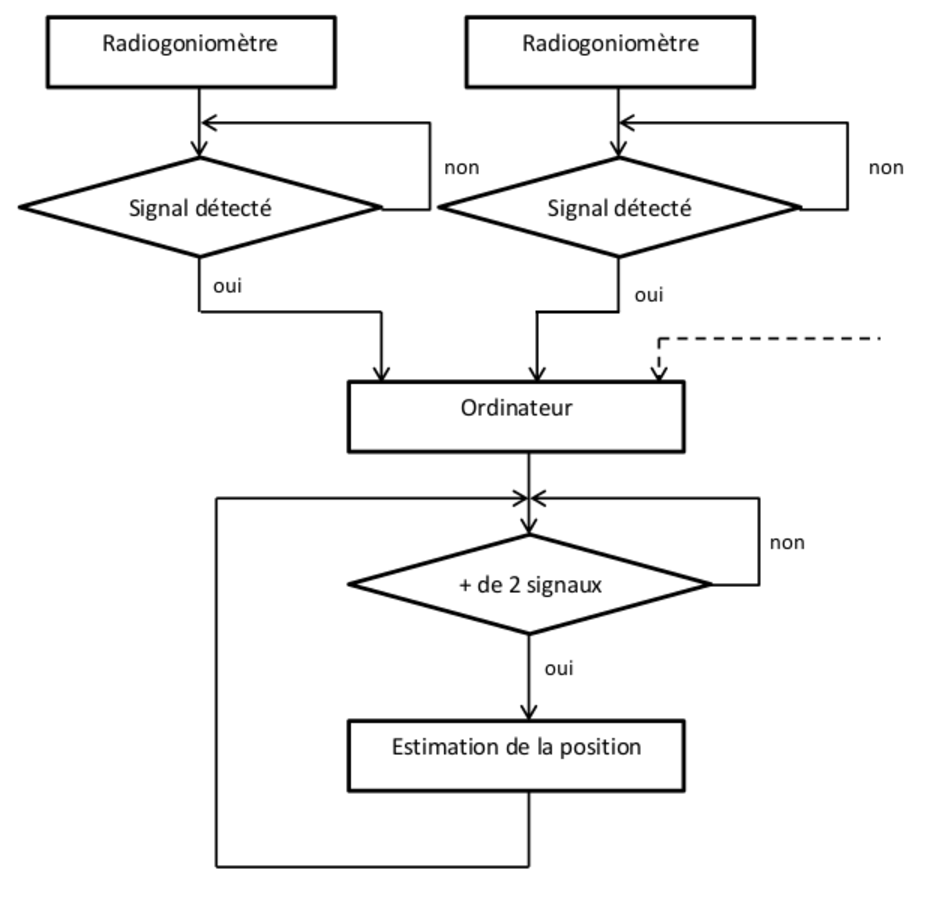
\includegraphics[width=0.8\textwidth]{SMART_logic}
\captionof{figure}{Schéma Logique du système}




%%% Local Variables: 
%%% mode: latex
%%% TeX-master: "rapport_analyse"
%%% End: 


\part{État de l'art}
\chapter{Radio-goniométrie}



Dans cette partie, nous allons nous attacher à étudier les différents types de goniométrie existant afin de retenir la solution la plus pertinente pour notre système. Cette étude redéfinira dans un premier temps le cadre de l’étude, puis suivra une explication de chaque technologie existante afin de conclure sur le choix que nous aurons retenu.
~\\

Généralement, un système de radiogoniométrie est composé de  :

\begin{itemize}
\item Un réseau de N capteurs avec ou sans processus de mise en forme des signaux d’antennes.

\item Un commutateur d’antenne
\item Un récepteur à plusieurs voies
\item Une unité de traitement du signal

\end{itemize}
~\\
De plus, la composition du système d’acquisition et les techniques de traitement du signal dépendent :
\begin{itemize}
\item  Des caractéristiques de l’onde à étudier
\item  Du type d’acquisition de l’information
\end{itemize}
~\\
Dans notre application, le système devra détecter une onde émise dans la gamme de fréquence UHF (2,4 GHz). Bien qu’existant dans le domaine de réalisation des radiogoniomètres, il n’est pas commun qu’un radiogoniomètre travail sur cette gamme de fréquence.

Les caractéristiques principales qui interviennent principalement dans le choix d’un radiogoniomètre sont:

\begin{itemize}
\item La précision de mesure angulaire (précision de la position obtenue)
\item La sensibilité (portée maximale du système) 
\item La vitesse de mesure
\item Le comportement en présence de plusieurs ondes dans la bande d’analyse
\item La susceptibilité du système
\end{itemize}
~\\
La spécificité de notre système est la cible à localisé. En effet, la source peut ne pas émettre en  continue et sur de très courtes période (inférieure à 1 seconde). Il nous faut donc un radiogoniomètre capable de réalisé la mesure en une fraction de seconde. La gestion de conservation de la donnée mesurée en attendant une valeur ultérieure sera gérée par l’ordinateur.


\section{Type de goniométrie}

\subsection{Goniométrie d'amplitude}

	La mesure se fait par repérage d’un maximum d’amplitude, d’un minimum d’amplitude, ou par comparaison de d’amplitude en sortie de deux diagrammes se recouvrant partiellement. La recherche du minimum d’amplitude à partir d’une antenne à cadre tournante est l’approche la plus ancienne. Un dipôle électrique est utilisé pour lever l’ambiguïté de 180\up{o} en formant un diagramme en cardioïde par sommation.
	
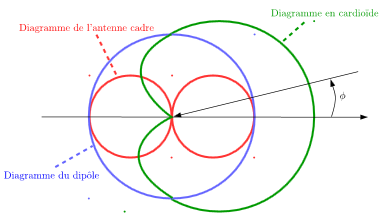
\includegraphics[width=\textwidth]{cardioide}
\captionof{figure}{diagramme en cardioide d’une antenne à cadre}
\parindent=15pt

	La formation de faisceaux est une technique plus récente issue des traitements radar. Elle utilise un ensemble de capteurs spatialement répartis. Les sorties d’antennes sont pondérées en phase puis sommées. Cette pondération est fonction du déphasage progressif d’une antenne à une autre, qui dépend de la direction d’arrivée et de la distance entre capteurs. Les pondérations permettent ainsi de remettre en phase les signaux et d’obtenir un diagramme avec un maximum dans la direction d’arrivée.
 Cette technologie est la plus ancienne. L’antenne utilisée était une antenne cadre et la gamme de fréquence étudiée était la HF et la VHF.

\subsection{Goniométrie Watson-Watt}
\label{Watson-Watt}

	Un radiogoniomètre Watson-Watt est un radiogoniomètre automatique. L’onde électromagnétique du système à localisé est reçue par deux antennes perpendiculaires dont le rapport des amplitudes est très proche de tan (l’une en sin et l’autre en cos). La goniométrie par interférométrie est considérée comme une technique plus performante comparée à celles citées précédemment. A la différence des deux techniques précédentes, le traitement n’est pas entièrement analogique. Des calculs numériques, plus ou moins complexes, sont nécessaires suivant la topologie de l’antenne utilisée. Elle n’a donc pu être mise en œuvre qu’à partir de l’arrivée des microprocesseurs.

\subsection{Goniométrie par interférométrie}

	La goniométrie par interférométrie est considérée comme une technique plus performante comparée à celles citées précédemment. A la différence des deux techniques précédentes, le traitement n’est pas entièrement analogique. Des calculs numériques, plus ou moins complexes, sont nécessaires suivant la topologie de l’antenne utilisée. Elle n’a donc pu être mise en œuvre qu’à partir de l’arrivée des microprocesseurs.
L’interférométrie utilise la mesure de la différence de phase de signaux délivrés par deux antennes proches illuminées par la même onde électromagnétique.

\subsection{Goniométrie par effet Doppler}

	Une antenne tournant autour d'un axe est placé dans le champ d'émission d'un émetteur de porteuse pure. A cause du mouvement de l'antenne, le signal reçu subit un effet Doppler qui se traduit par une modulation FM du signal reçu. La fréquence instantanée du signal augmente quand l’antenne se rapproche de la direction d’arrivée du signal et décroît lorsqu’elle s’en éloigne. En effectuant une démodulation FM, on peut détecter la direction de provenance des ondes en comparant la phase du signal obtenu et celle de la rotation angulaire de l’antenne. 
Afin d'éviter de devoir faire tourner mécaniquement l'antenne, on peut en disposer plusieurs en cercle et les commuter successivement.

\section{Selection de la technologie}

	Après étude des différentes technologies existantes, nous nous baserons sur une étude comparative menée par le site F1LVT.

~\\	
	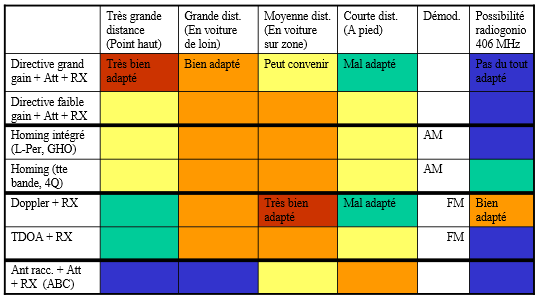
\includegraphics[width=\textwidth]{tableauTechnologies}
	\captionof{figure}{Radiogoniométrie VHF-UHF pour les bandes aviation et les bandes RA}
\parindent=15pt
~\\

	Ce tableau compare plusieurs technologies ainsi que leurs caractéristiques. Dans le cadre d’un système devant opéré en extérieur sur zone (environ de zone industriel ou de central électrique ) nous retenons le goniomètre Doppler.





%%% Local Variables: 
%%% mode: latex
%%% TeX-master: "rapport_analyse"
%%% End:

\chapter{Composants}


\section{Antennes}

\subsubsection{Principes généraux}

	Les goniomètres utilisent les ondes radioélectriques pour pouvoir localiser la direction d'une source d'émissions. Chaque type de goniomètre utilisera une ou plusieurs antennes pour pouvoir analyser les caractéristiques de l'onde reçue. 
	Le fonctionnement de ces antennes est décrit par les lois de l'électromagnétisme. Chaque onde électromagnétique possède une composante électrique et une composante magnétique. La composante ou champ électrique de cette onde fera apparaitre des variations de potentiel dans l'antenne dont l'amplitude et la fréquence seront directement liés à l'onde qui les a généré. Leur analyse permettra de récupérer les caractéristiques de l'onde reçue et d'en extraire les informations pertinentes pour le système équipé de l'antenne.
	
\subsection{Antennes en Radiogoniométrie}

	En radiogoniométrie il est possible de travailler avec plusieurs types d'antennes. La méthode la plus simple pour déterminer la direction d'une onde sera d'utiliser une antenne à ouverture dite faible et de la faire pivoter pour pouvoir déterminer la direction du maximum d'émission. Une antenne circulaire ou rectangulaire pourra convenir. Parfois le type de goniomètre utilisé déterminera le choix de l'antenne. Par exemple dans le cas d'un radiogoniomètre de type Watson-Watt plusieurs solutions sont envisageables: 
	
\begin{itemize}

\item l'utilisation de deux antennes circulaires ou rectangulaires.

\item L'utilisation d'une antenne dite "Adcock" qui est une combinaison d'antennes monopoles ou dipolaires. 

\end{itemize} 

	Dans le cadre de notre projet, nos recherches nous ont conduit à choisir un goniomètre Doppler. Ce type de goniomètre utilise au minimum quatres antennes monopoles ou dipolaires disposées en croix autour d'une antennes de référence omnidirectionnelle (une antenne monopole est souvent utilisée). Pour un nombre d'antennes supérieur celles-ci seront disposées en cercle à intervalle régulier autour de l'antenne de référence.	
	
	En théorie deux antennes pourraient suffire. Si on parvenait à mettre en rotation une antenne omnidirectionelle autour de l'antenne de référence suffisamment rapidement le goniomètre Doppler fonctionnerait. Il est toutefois beaucoup plus simple d'utiliser un ensemble d'antennes disposées en cercle et "d'écouter" successivement chaque antenne à l'aide d'un commutateur pour simuler cette rotation.
	
\subsection{Système d'antennes retenu}

	Le goniomètre Montréal possède cinq antennes, quatre disposées en croix et une antenne centrale connectées au système électronique de traitement. Les antennes sont reliées à un commutateur permettant de sélectionner successivement les antennes de la croix. Le système est dimensionné autour de trois critères : 
	
\begin{itemize}

\item La bande de fréquence surveillée par les antennes : On utilisera ici des antennes monopoles (quart d'onde) adaptées au 2,4GHz

\item Le rayon d'écartement des antennes (distance entre les quatres antennes de la croix et l'antenne de référence) : Si ce rayon est trop faible les écarte de fréquence seront plus difficiles à remarquer et le bruit électromagnétique peut être plus gênant lors de la mesure.


\item La vitesse de commutation des antennes.

\end{itemize}

Deux des paramètres sont fixés à l'installation du dispositif. Les formules suivantes permettent de déterminer le paramètre manquant.

\begin{equation}
dF = \frac{w*r*f_c}{c}
\end{equation}

et

\begin{equation}
f_r = \frac{dF*1879.8}{R*f_c}
\end{equation}

Les antennes utilisées pour le montage pourront être celles utilisées dans l'aéromodélisme et sur les drones amateurs qui utilisent dans leur grande majorité la bande des 2,4 GHz.

Les modèles d'antennes suivants pourraient convenir :

\begin{itemize}

\item FrSky 2.4G V8 Series 5db module Antenna

\item Orange 2.4G Antenna 2db (Extended wire)

\end{itemize}

Il est aussi possible de les concevoir nous même en respectant les dimensions ( 3,125 cm pour une monopole, 6.25 cm pour une dipôle)

%%% Local Variables: 
%%% mode: latex
%%% TeX-master: "rapport_analyse"
%%% End:



%%%% CONCLUSION %%%%%%%%%

\chapter*{Conclusion}
\addcontentsline{toc}{chapter}{Conclusion}
Bien que sommaire, cette première analyse comprenant de la recherche bibliographique, de la veille technologique et de l'analyse fonctionnelle, nous permet de nous recentrer sur l'essentiel. Le domaine de la localisation de drone étant en plein essor, il est primordial de se concentrer sur un type de détection et d'avancer pas à pas.

Nous allons donc, dès à présent, nous attacher à la compréhension de la radiogoniométrie ainsi qu'à poursuivre la veille technologique afin de retenir les bonnes solutions de détection.

\newpage

%%%% ANNEXE %%%%%%%%%%%%

\part*{Annexe}
\appendix
\nocite{*}

\chapter{Organisation du travail}


\section{Méthode de travail}

Nous avons cherché au mieux à répartir notre travail. Pour cela nous avons défini 3 grands axes de travail à l'issue de cette étude fonctionnelle.
\begin{itemize}
\item Dans un premier temps nous allons réaliser l'état de l'art.
\item Dans un deuxième temps nous étudierons la phase de réalisation.
\item Enfin nous testerons notre projet dans des conditions réelles.
\end{itemize}
~\\

Tout au long de ce projet nous avons choisi de réaliser notre travail en divisant notre équipe en 3 groupes de travail distincts formés respectivement de D'Acremont - Cotten, Legay - Rigaud, et Kenaan - Shehade. Notamment lors de l'état de l'art, ces groupes vont réaliser des recherches par binômes pour ensuite redistribuer les informations grâce aux outils mis à notre disposition (nous avons détaillé ces outils plus loin).
~\\

De plus, nous avons décidé lors de la phase de conception de diviser ce travail en plusieurs sous ensembles que nous définirons plus tard et qui seront chacun d'eux testés indépendamment, à l'image de tests unitaires en programmation.



\section{Outils utilisés}

Lors de notre projet nous avons choisi d'utiliser plusieurs outils de travail en collaboration.

\begin{itemize}
\item Nous utilisons Office 365. Nous avons créé un groupe de travail où nous partageons des fichiers et envoyons des mails de manière centralisée.
\item Nous utilisons également \LaTeX~pour la rédaction de nos rapports.
\item Nous pensons finalement utiliser Git et GitHub lors de notre phase de conception. Nous avons pour cela crée un projet sur GitHub.
\item Après plusieurs difficultés, nous avons réussi à utiliser Framaboard du groupe Framasoft pour gérer notre projet.
\end{itemize}

~\\
~\\

\subsection{Framaboard}
\begin{center}
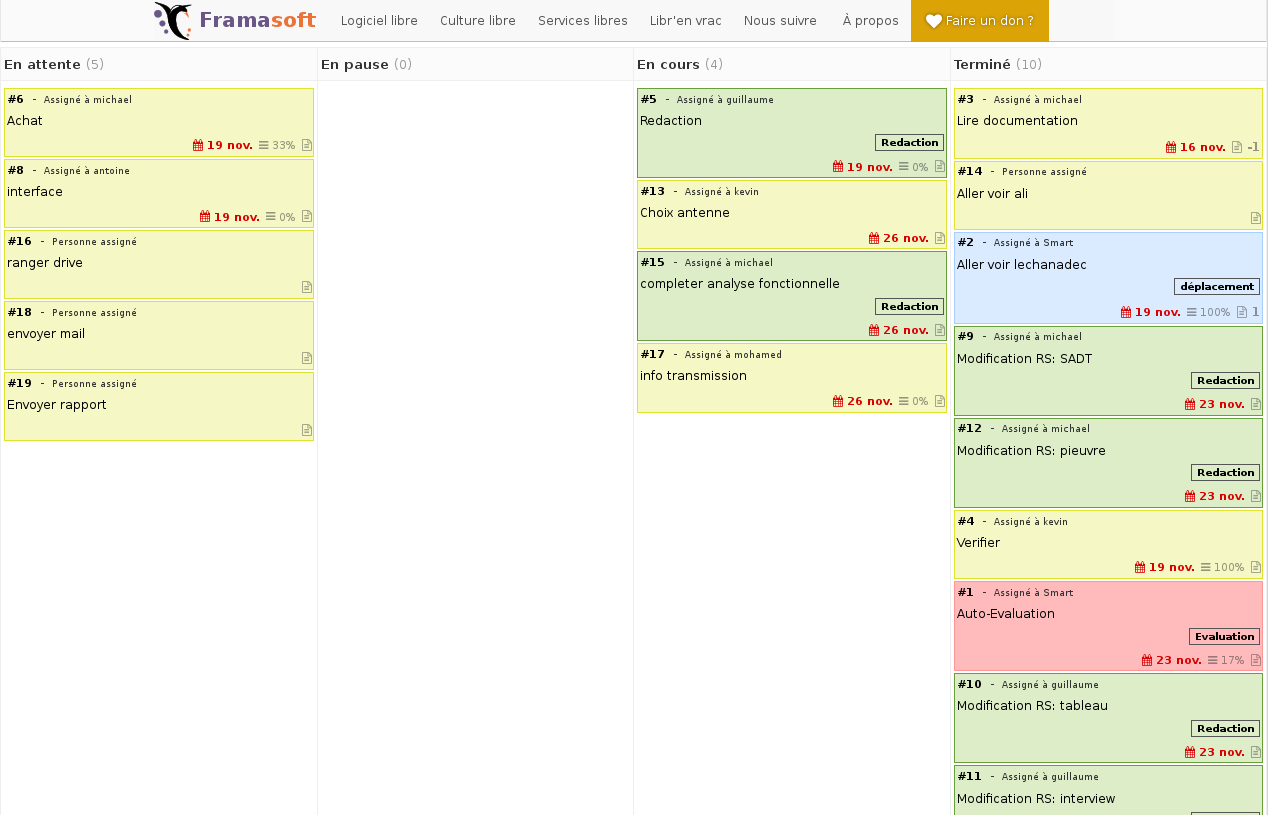
\includegraphics[width=0.9\textwidth]{framaboard}
\captionof{figure}{Impression d'écran de notre Framaboard}
\end{center}
Il est possible d'avoir accès en lecture à notre page Framaboard en cliquant  \textit{\href{https://smart.framaboard.org/?controller=board&action=readonly&token=ab1e20bb26472df067dc24cbd84d9b28eea71bfd68bdea07ab5a9b555ce0}{ici}}

\subsection{GitHub}
\begin{center}
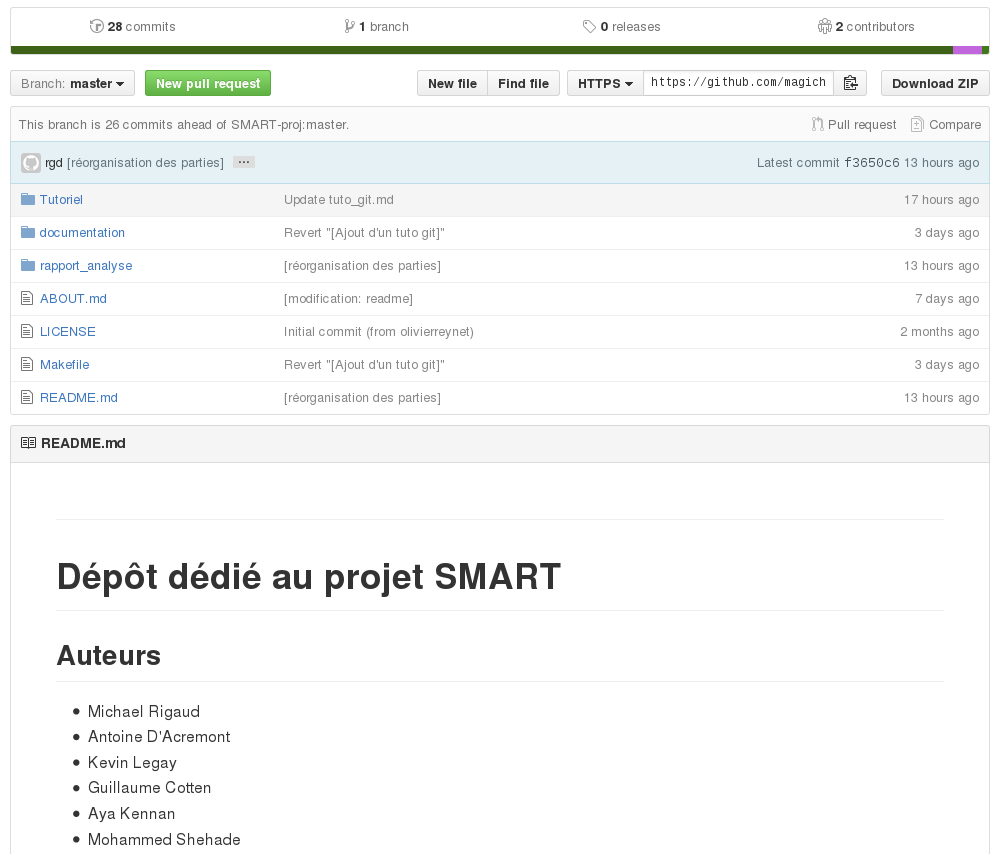
\includegraphics[width=0.9\textwidth]{github}
\captionof{figure}{Impression d'écran de notre GitHub}
\end{center}
Il est possible d'avoir accès à notre page GitHub en cliquant  \textit{\href{https://github.com/magichal/SMART}{ici}}






  


%%% Local Variables: 
%%% mode: latex
%%% TeX-master: "rapport_analyse"
%%% End: 

\chapter{Le Montréal 3V2}
\label{montreal}

Nous allons ici présenter la solution sur laquelle nous nous appuyons pour réaliser notre propre radiogoniomètre à effet Doppler, le Montréal 3V2.
Pour réaliser cette documentation nous nous sommes appuyé sur la documentation trouvé sur le site f1lvt \cite{montreal}

\section{Évolution du Montréal}

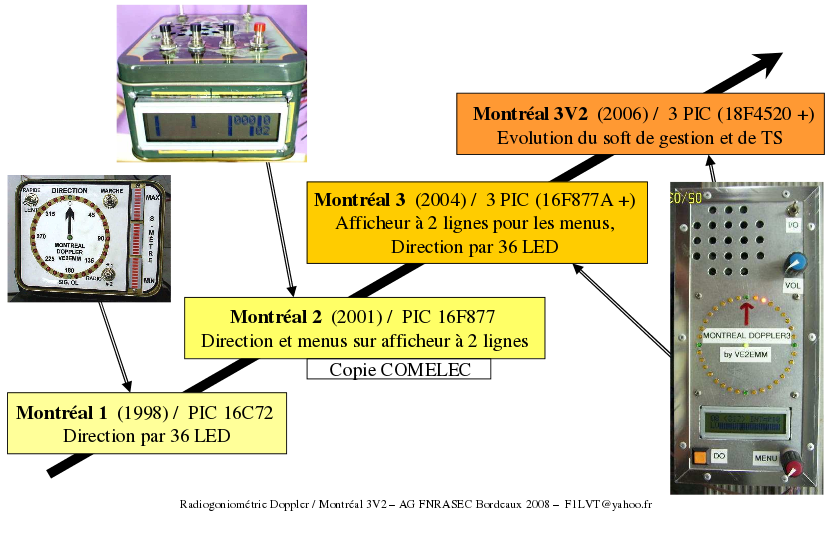
\includegraphics[width=\textwidth]{evolution}
\captionof{figure}{Evolution du Montréal}

\section{Avantages du Montréal 3v2}

\begin{center}
  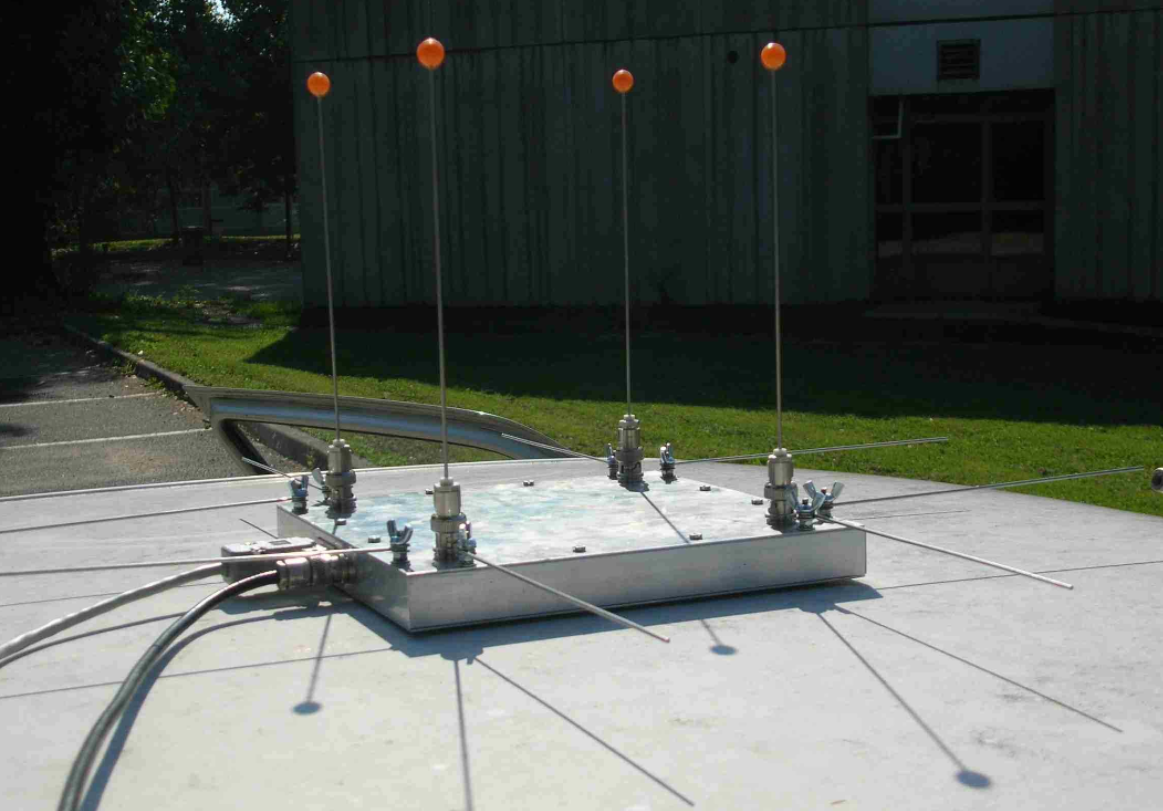
\includegraphics[width=0.5\textwidth]{montreal}
  \captionof{figure}{Photographie prise du Montréal 3v2}
\end{center}

\parindent=15pt
Le Montréal 3v2 sert principalement à l'FNRASEC\footnote{Fédération Nationale des Radioamateurs au service de la Sécurité Civile, agrée de sécurité civile} et aux chasseurs d'onde amateurs. Ce radiogoniomètre est utilisé pour la détection de balise de détresse de 406MHz.

%Parmi ses avantages, on peut noter qu'il est facile à construire, son prix , et il est simple d'utilisation. 

Un des intérêts majeurs du Montréal 3-V2, c'est sa capacité de localiser des signaux très courts, son prix de revient est très raisonnable,son traitement très rapide et la mise en mémoire automatique du dernier relevé. On peu aussi noter qu'il est simple d'utilisation grâce a son affichage à 36LED disposé en cercle et qui indique la direction. De plus une LED centrale est indique le fonctionnement; verte la direction affichée est bonne, rouge le signal est insuffisant, la direction reste alors figée dans la dernière bonne direction reçue.

%on peut noter son affichage à 36 LED qui indique la direction de manière clair et efficace, et un réglage facilité par son écran LCD ou encore son filtre à capa commutée à très faible largeur de bande (0,5 Hz).

\section{Caractéristiques}

Le Montréal 3v2 est un radiogoniomètre à effet Doppler, il possède donc toutes les caractéristiques associé a ce type de radiogoniomètre.
~\\

\begin{tabular}{ l l l}
Fréquences & distance & moyenne portée\\
 & gamme & 50MHz-1.3GHz\\
 & démodulation & FM\\
Affichage & LED & 36LED\\
& écran & LCD en 2 lignes\\
Filtre & capa & très faible largeur de bande (0.5Hz)\\
Coût & & estimé à 50\euro \\
\end{tabular}


\section{Fonctionnement}
La partie centrale contient les circuits d'amplification et de commutation. Les 4 brins verticaux (les brins actifs) se fixent par BNC.

Les antennes sont alimentées de façon séquentielle pour imiter une antenne en rotation. Une fois que les antennes ont capté les ondes provenant du drone, il faut faire une démodulation et enlever tous les bruits.


Un système à LED permet de visualiser la composante continue qui passe dans les antennes. A partir du boîtier Doppler et de son menu de test, on peut ainsi vérifier individuellement chaque antenne. Ceci permet soit de faire fonctionner le système Doppler avec une antenne sur 4 %(fonctionnement conforme à la théorie avec une seule antenne tournante)
, soit avec 3 antennes sur 4. %(ce qui inverse le signal Doppler à 500 Hz ; mais ça fonctionne aussi bien voire mieux).


Trois microcontrôleurs Pics sont utilisés un 16F628A pour l'affichage, un 16F877A pour le circuit principal et un 12F675 comme diviseur de fréquence.

Ce Doppler est la version la plus récente et la plus performante de la série. Il commute les antennes et il affiche la direction mesurée sur la boussole à 36 LED. 
~\\

Une présentation plus détaillé du fonctionnement interne des PIC est fournie dans la figure suivante:


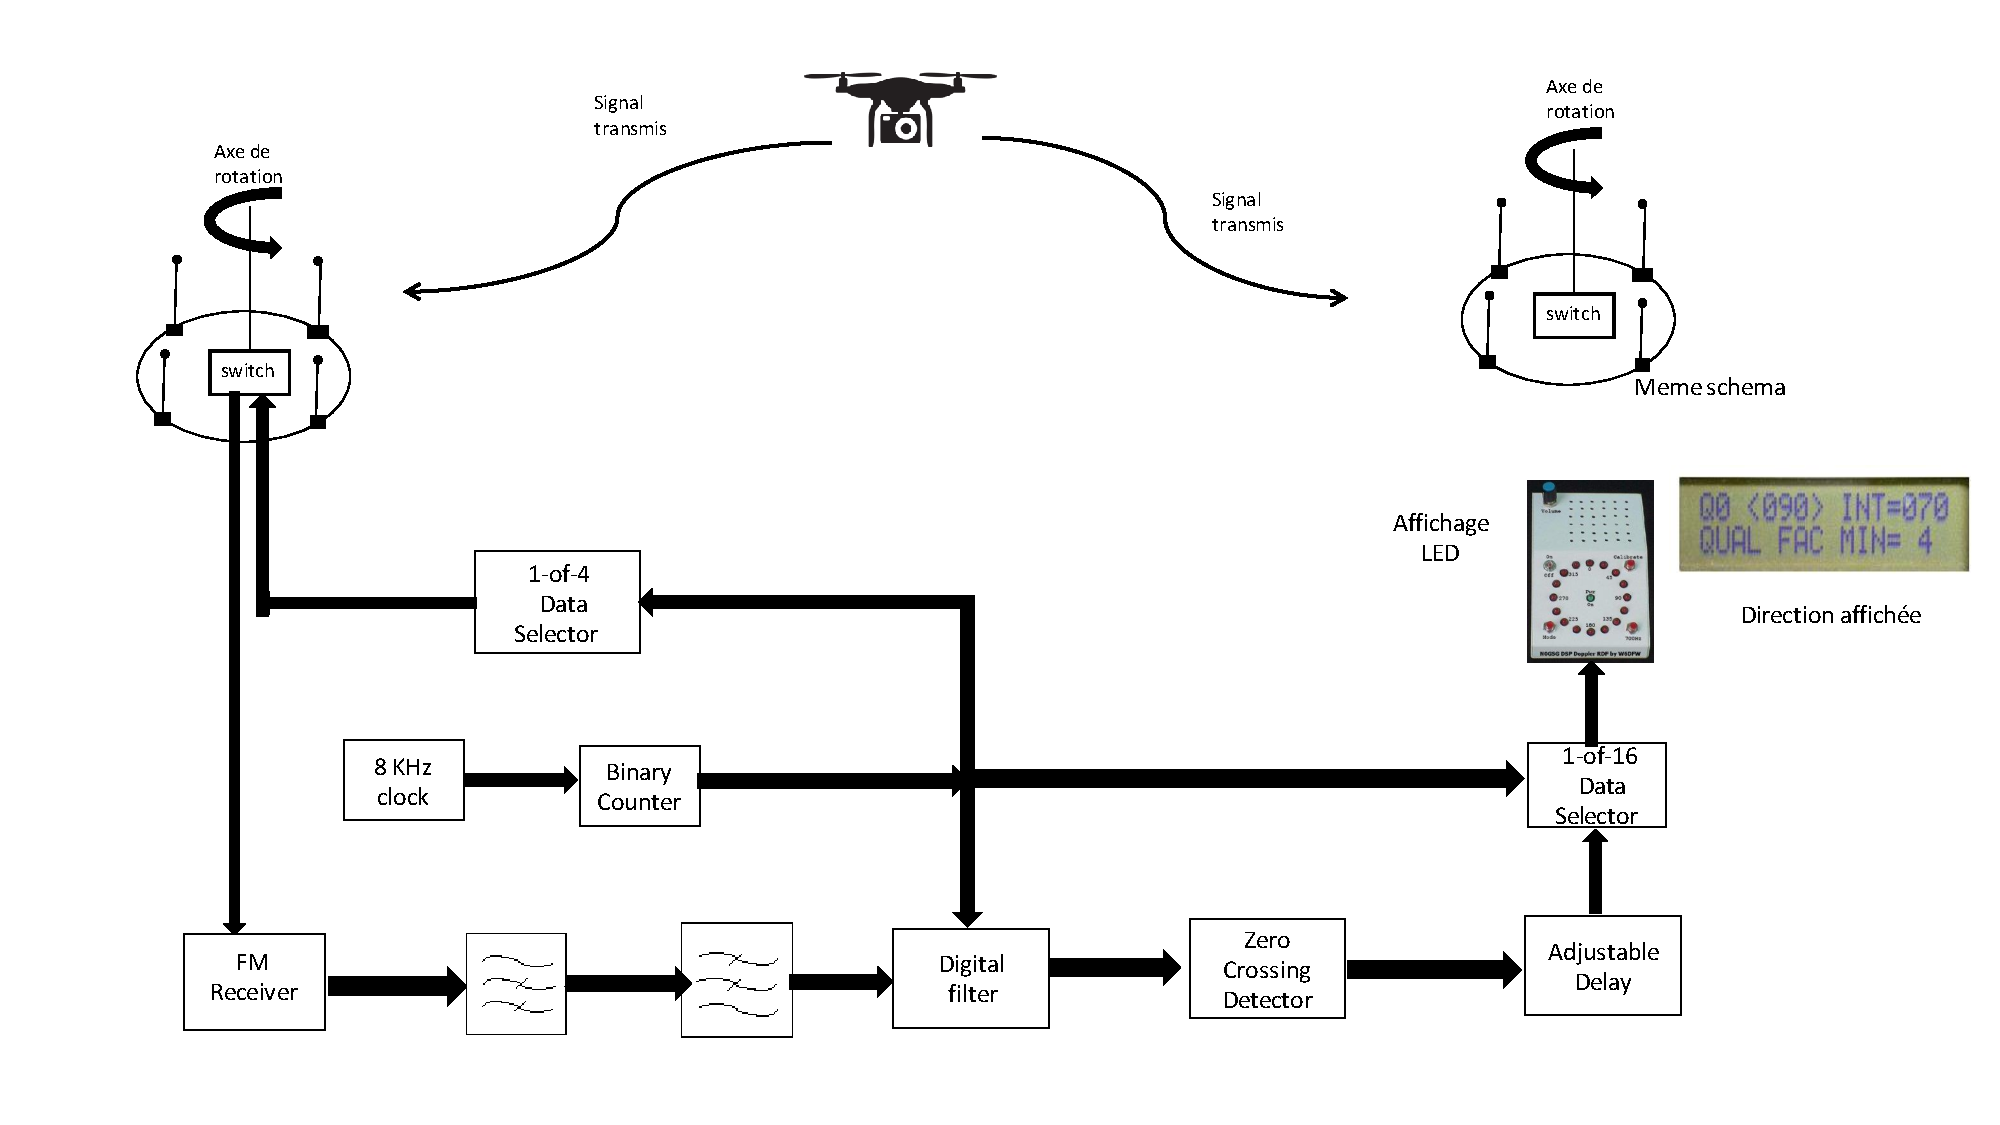
\includegraphics[width=\textwidth]{Presentation1}
\captionof{figure}{Présentation détaillé du système}



\section{Schéma bloc}

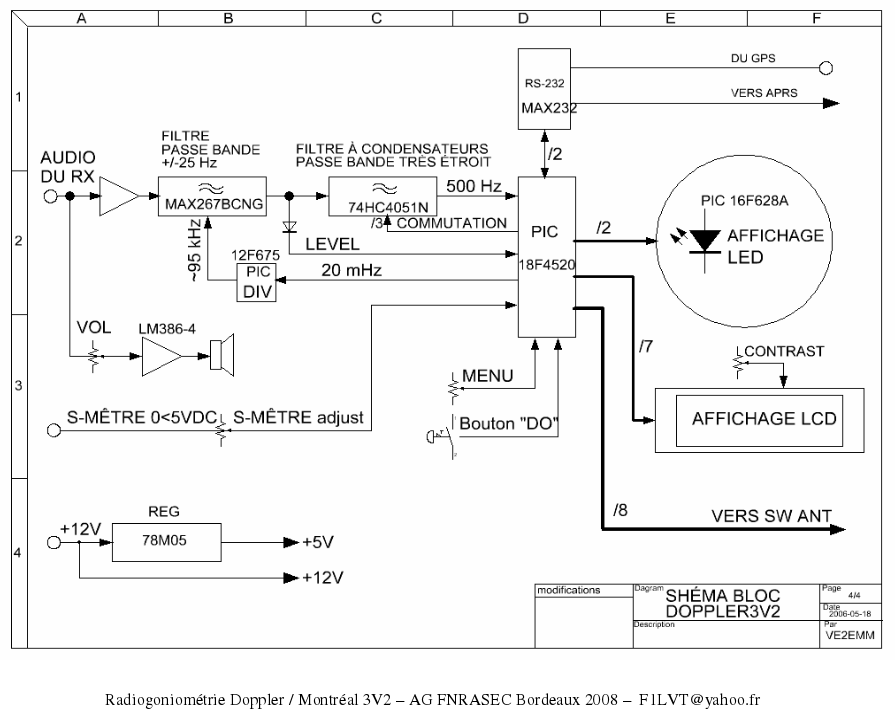
\includegraphics[width=\textwidth]{schemaBloc}
\captionof{figure}{Schéma bloc du Montréal 3v2}

\section{Liste des composants}
Voici la liste des composants pour la construction du Montréal 3v2:

\begin{tabular}{ l l l}

IC30&          LM386N-4&                  Ampli BF\\
IC50&          MAX267BCNG&          Filtre\\
IC51& PIC  12F675-I/P& PIC \\
IC52&          74HC4051N&               Filtre\\
IC53&          MAX492CPA &            Ampli Op\\
IC70& PIC  18F4520-I/P& PIC\\
VR20 &       7805 TO-220  &            Régulateur\\
X70&           20 MHz  HC49&           Quartz\\
D50&           1N5819       &                Diode Schottky\\
LCD20&      LCD 2X16,&                 Afficheur 2 lignes de 16 car.\\
IC1& PIC16F628A-I/P& PIC\\
LED1 - LED36& ø3mm, Rouge et/ou Vert&\\
LED37&                        3 ou 5mm Bicolore Rouge/Verte &\\
FB1 - FB8&                   Ferrites\footnote{+ composants passifs : Résistances, Condensateurs.}&\\
IC100&        = MAX232ACPE&        en option\\
Q100 &        = 2N2222 TO-92&\\
\end{tabular}
\captionof{figure}{Liste des composants}


%%% Local Variables: 
%%% mode: latex
%%% TeX-master: "rapport_analyse"
%%% End: 


\newpage
\listoffigures
\printindex
\bibliographystyle{plain}
\bibliography{biblio}

\end{document}
%%%%%%%%%%%%%%%%% FIN DU DOCUMENT
